\section{Einführung}
\section{Versuch}
Im Folgendem werden die Kennlienen von verschieden Bauteilen mit dem Aufbau \ref{fig:aufbau} bestimmt. Sämtliche Messwerte für die Spannung wurden mit einem Messfehler von $\Delta U = V$ bzw. $\Delta I = mA$ aufgenommen.
\begin{figure}[H]
	\centering
	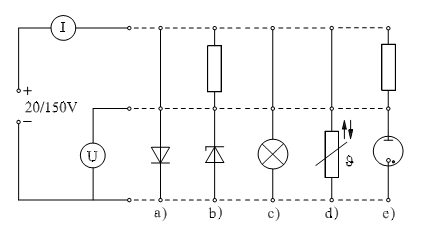
\includegraphics[width=.8\textwidth]{Aufbau.png}
	\caption{Messaufbau für unterschiedliche Leiter}
	\label{fig:aufbau}
\end{figure}
\subsection{Diode in Durchlassrichtung}
Wie in Abbildung \ref{fig:aufbau} a) gezeigt wird der Strom für unterschiedliche Spannung gemessen, um daraus eine U-I-Kennlinie zu ermitteln.

\begin{figure}[H]
\centering
\begin{tikzpicture}
  \begin{axis}[
    width=15 cm,
    height=9 cm,
    xmin=0, xmax=0.8,
    ymin=-1, ymax=60,
    xlabel={$U$ [\si{mV}]},
    ylabel={$I$ [\si{mA}]},
    domain=0:0.8,
    cycle list name=color list,
    legend entries={Messwerte, $a\cdot b^x$},
    legend pos=north west
  ]
  \addplot+ plot [only marks,mark=x]  table {Diode.txt};
  \addplot+ plot [samples=500, mark=none] {5.61784*10^(-7)*(1.69598*10^11)^x};
  \end{axis}
\end{tikzpicture}
\caption{Messwerte und Fit für eine Diode in Durchlassrichtung}
\label{fig:diode}
\end{figure}
Aufgrund des anscheinend exponentiellen Verlaufs der Messwerte wurde mit \emph{gnuplot} nach dem \emph{least-squares}-Verfahren die Werte gegen die Funktion $f(x)=a\cdot b^x$ gefittet. Ausgabe:
\begin{table}[H]
  \centering
  \begin{tabular}{c | c | c }
    Variabel   & Wert & Unsicherheit\\ \hline
    a & $\num{5.61784d-7}$ & $\pm\num{3.084d-8}$ \\
    b & $\num{1.69598d+11}$ & $\pm\num{1.319d+10}$
  \end{tabular}
  \caption{Linearer Fit zu Abbildung \ref{fig:diode}}
  \label{tab:fitdiode}
\end{table}
\subsection{Zenerdiode}
Wie in Abbildung \ref{fig:aufbau} b) gezeigt wird der Strom für unterschiedliche Spannung gemessen, um daraus eine U-I-Kennlinie zu ermitteln. Dies wird jedoch einmal mit einer Polung in Durchlassrichtung und einmal in Sperrrichtung getan.
\begin{figure}[H]
\centering
\begin{tikzpicture}
  \begin{axis}[
    width=15 cm,
    height=9 cm,
    xmin=0, xmax=6,
    ymin=-1, ymax=30,
    xlabel={$U$ [\si{V}]},
    ylabel={$I$ [\si{mA}]},
    domain=0:6,
    cycle list name=color list,
    legend entries={Messwerte, $a\cdot b^x$},
    legend pos=north west
  ]
  \addplot+ plot [only marks,mark=x]  table {Diodesperr.txt};
  \addplot+ plot [samples=500, mark=none] {1.50271*10^(-7)*(42.7533)^x};
  \end{axis}
\end{tikzpicture}
\caption{Messwerte und Fit für eine Zenerdiode in Sperrrichtung}
\label{fig:diodesperr}
\end{figure}
Aufgrund des anscheinend exponentiellen Verlaufs der Messwerte wurde mit \emph{gnuplot} nach dem \emph{least-squares}-Verfahren die Werte gegen die Funktion $f(x)=a\cdot b^x$ gefittet. Ausgabe:
\begin{table}[H]
  \centering
  \begin{tabular}{c | c | c }
    Variabel   & Wert & Unsicherheit\\ \hline
    a & $\num{1.50271d-7}$ & $\pm\num{5.433d-8}$ \\
    b & $\num{42.7533}$ & $\pm\num{3.073}$
  \end{tabular}
  \caption{Linearer Fit zu Abbildung \ref{fig:diodesperr}}
  \label{tab:fitdiodesperr}
\end{table}
\begin{figure}[H]
\centering
\begin{tikzpicture}
  \begin{axis}[
    width=15 cm,
    height=9 cm,
    xmin=0, xmax=0.8,
    ymin=-1, ymax=40,
    xlabel={$U$ [\si{V}]},
    ylabel={$I$ [\si{mA}]},
    domain=0:0.8,
    cycle list name=color list,
    legend entries={Messwerte, $a\cdot b^x$},
    legend pos=north west
  ]
  \addplot+ plot [only marks,mark=x]  table {Diodedurch.txt};
  \addplot+ plot [samples=500, mark=none] {3.08803*10^(-11)*(9.72068*10^16)^x};
  \end{axis}
\end{tikzpicture}
\caption{Messwerte und Fit für eine Zenerdiode in Durchlassrichtung}
\label{fig:diodedurch}
\end{figure}
Aufgrund des anscheinend exponentiellen Verlaufs der Messwerte wurde mit \emph{gnuplot} nach dem \emph{least-squares}-Verfahren die Werte gegen die Funktion $f(x)=a\cdot b^x$ gefittet. Ausgabe:
\begin{table}[H]
  \centering
  \begin{tabular}{c | c | c }
    Variabel   & Wert & Unsicherheit\\ \hline
    a & $\num{3.08803d-11}$ & $\pm\num{3.759d-12}$ \\
    b & $\num{9,72068d16}$ & $\pm\num{1.673d16}$
  \end{tabular}
  \caption{Linearer Fit zu Abbildung \ref{fig:diodedurch}}
  \label{tab:fitdiodedurch}
\end{table}
\subsection{Glühlampe}
Wie in Abbildung \ref{fig:aufbau} c) gezeigt wird der Strom für unterschiedliche Spannung gemessen, um daraus eine U-I-Kennlinie zu ermitteln.

\begin{figure}[H]
\centering
\begin{tikzpicture}
  \begin{axis}[
    width=15 cm,
    height=9 cm,
    xmin=0, xmax=14,
    ymin=0, ymax=60,
    xlabel={$U$ [\si{V}]},
    ylabel={$I$ [\si{mA}]},
    domain=0:14,
    cycle list name=color list,
    legend entries={Messwerte, $a\sqrt{x}$},
    legend pos=north west
  ]
  \addplot+ plot [only marks,mark=x]  table {Lampe.txt};
  \addplot+ plot [samples=500, mark=none] {14.9315*sqrt(x)};
  \end{axis}
\end{tikzpicture}
\caption{Messwerte und Fit für eine Lampe}
\label{fig:Lampe}
\end{figure}
Aufgrund des anscheinend Wurzel artigem Verlaufs der Messwerte, besonders im Bereich bis $3V$, wurde mit \emph{gnuplot} nach dem \emph{least-squares}-Verfahren die Werte gegen die Funktion $f(x)=a\cdot\sqrt{x}$ gefittet. Ausgabe:
\begin{table}[H]
  \centering
  \begin{tabular}{c | c | c }
    Variabel   & Wert & Unsicherheit\\ \hline
    a & $\num{14,9315}$ & $\pm\num{0,2092}$ \\
   
  \end{tabular}
  \caption{Linearer Fit zu Abbildung \ref{fig:Lampe}}
  \label{tab:fitlampe}
\end{table}
\subsection{NTC}
Wie in Abbildung \ref{fig:aufbau} d) gezeigt wird der Strom für unterschiedliche Spannung gemessen, um daraus eine U-I-Kennlinie zu ermitteln. Dabei muss nach jeder Spannungserhöhung gewartet werden, bis sich der Temperaturgradient abgebaut hat. 

\begin{figure}[H]
\centering
\begin{tikzpicture}
  \begin{axis}[
    width=15 cm,
    height=9 cm,
    xmin=0, xmax=8,
    ymin=0, ymax=60,
    xlabel={$U$ [\si{V}]},
    ylabel={$I$ [\si{mA}]},
    domain=0:8,
    cycle list name=color list,
    legend entries={Messwerte, $ax^2+bx+c$},
    legend pos=north west
  ]
  \addplot+ plot [only marks,mark=x]  table {NTC1.txt};
  \addplot+ plot [samples=500, mark=none] {0.316693*x^2-0.0533435*x+1.05214};
  \end{axis}
\end{tikzpicture}
\caption{Messwerte und Fit für eine NTC-Widerstand}
\label{fig:ntc}
\end{figure}
Aufgrund des anscheinend quadratischem Verlaufs der Messwerte wurde mit \emph{gnuplot} nach dem \emph{least-squares}-Verfahren die Werte gegen die Funktion $f(x)=a\cdot x^2+b\cdot x+c$ gefittet. Beim Fitten wurde der letzte Messwert nicht betrachtet, da er vollkommen aus dem Verlauf der Werte herausfällt. Dies ist auf ein Versagen der Leistung des Netzgeräts zurückzuführen. Ausgabe:
\begin{table}[H]
  \centering
  \begin{tabular}{c | c | c }
    Variabel   & Wert & Unsicherheit\\ \hline
    a & $\num{0,316693}$ & $\pm\num{0,05691}$ \\
    b & $\num{-0,0533435}$ & $\pm\num{0,4446}$ \\
    c & $\num{1,05214}$ & $\pm\num{0,6146}$ \\
  \end{tabular}
  \caption{Linearer Fit zu Abbildung \ref{fig:Lampe}}
  \label{tab:fitlampe}
\end{table}


\section{Diskussion}
\notecite{anleitung-ws2014}
